% 1986 年上海卷文史类第 7 题图 1：折叠前的直角三角形
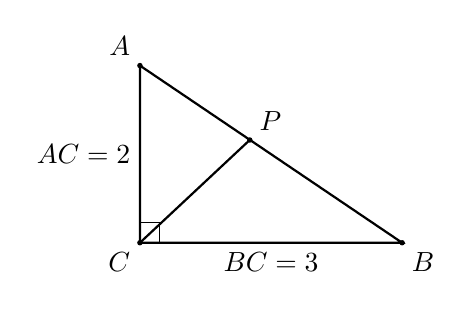
\begin{tikzpicture}[scale=0.9,>=stealth]
  \coordinate (C) at (0,0);
  \coordinate (A) at (0,2.5);
  \coordinate (B) at (3.7,0);
  \coordinate (P) at (1.55,1.45);
  \draw[thick] (A)--(C)--(B)--cycle;
  \draw[thick] (C)--(P);
  \draw (0,0.28)--(0.28,0.28)--(0.28,0);
  \fill (A) circle (1.1pt) node[above left] {$A$};
  \fill (B) circle (1.1pt) node[below right] {$B$};
  \fill (C) circle (1.1pt) node[below left] {$C$};
  \fill (P) circle (1.1pt) node[above right] {$P$};
  \node[left] at (0,1.25) {$AC=2$};
  \node[below] at (1.85,0) {$BC=3$};
\end{tikzpicture}
